\section{Traffic Engineering}
\label{chapter:srte}

\textbf{Why?} Simple, automated and scalable:
\begin{itemize}
    \item no core state
    \item no tunnel interface
    \item no head-end a-priori configuration
    \item no head-end a-priori steering
\end{itemize}

\noindent
Multi-Domain:
\begin{itemize}
    \item SR-PCE: Path Computation Element
    \item Binding-SID for scale
\end{itemize}

\noindent
\textbf{What?} SR Policies

Tuple of \ttfamily (head-end, color, end-point) \rmfamily uniquely identifies an SR Policy.
Head-end: Router originating the SR policy (source).
Color: a numerical value to differentiate multiple policies between the same pair of nodes. (Green: low-cost policy, red: low-delay policy)

\begin{figure}[h]
    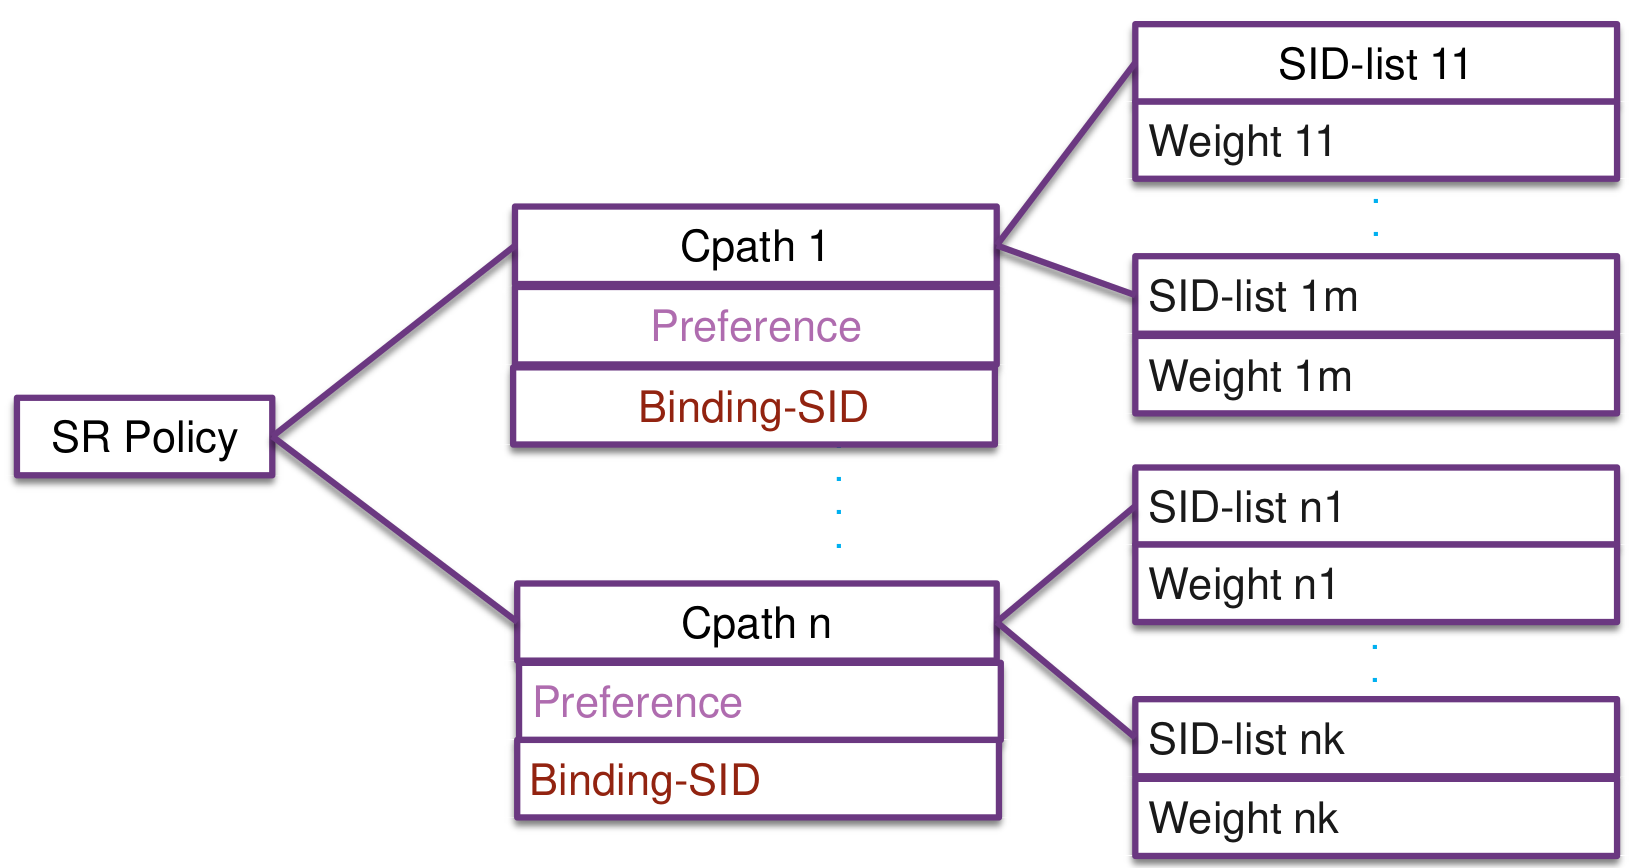
\includegraphics[width=\textwidth]{sr-policies.png}
    \caption{Structure of an SR Policy}
\end{figure}

\begin{itemize}
    \item An SR Policy consists of 1-n candidate paths
    \item An SR Policy instantiates one single candidate path in RIB/FIB 
    \item An SR Policy and all its candidate paths are associated with a single Binding-SID
    \item Binding SID may change at  some point In time, true ID of SR Policy is its tuple
    \item \emph{Binding SID installs an entry in the forwarding table to steer packets to use this policy}
\end{itemize}

\noindent
A candidate path
\begin{itemize}
    \item is either:
    \begin{itemize}
        \item dynamic, so that it contains an optimization objective and constraints
        \item explicit, so that it contains a single or a set of weighted SID lists.
    \end{itemize}
    \item has a preference
    \item is valid if it is usable:
    \begin{itemize}
        \item not empty
        \item first SID is resolvable (to account for multi-domain)
    \end{itemize}
\end{itemize}

\noindent
Candidate Path selection happens if 
\begin{itemize}
    \item it is valid 
    \item preference is highest    
\end{itemize}

\noindent
Validity of Policies is updated upon any network topology change.
Traffic steered into an SR Policy path is load-shared over all SID-lists of the path $\rightarrow$ weighted ECMP based on SID List Weight 

\subsection{Traffic Engineering Controller}
Usually, any head-end is able to compute SR-TE paths with certain optimization requirements. Still, a central view of the whole segment routing domain is necessary for several special use cases.
\begin{itemize}
    \item Disjoint paths: two head-ends explicitly request calculation of disjoint paths from the PCE. The controller can keep track of this requirement also in case of topology changes.  
    \item Inter-domain routing: The SR-TE database is natively multi-domain capable. Information about other SR domains is available via BGP Peering links (BGP-LS).
    \item Bandwidth brokering: The centralized bandwidth broker receives the bandwidth-related request from the individual routers, keeps
    track of the available bandwidth in the network and routes the requests accordingly.
\end{itemize}

\textbf{PCC -- Path Computation Client (Headend)}

Any device that receives SR paths externally instead of calculating them itself.
Candidate paths can be distributed via 
\begin{itemize}
    \item \textbf{PCEP:} Path Computation Element Protocol
    \item CLI configuration
    \item NETCONF / RESTCONF
    \item BGP 
\end{itemize}

\begin{figure}[h]
    \centering
    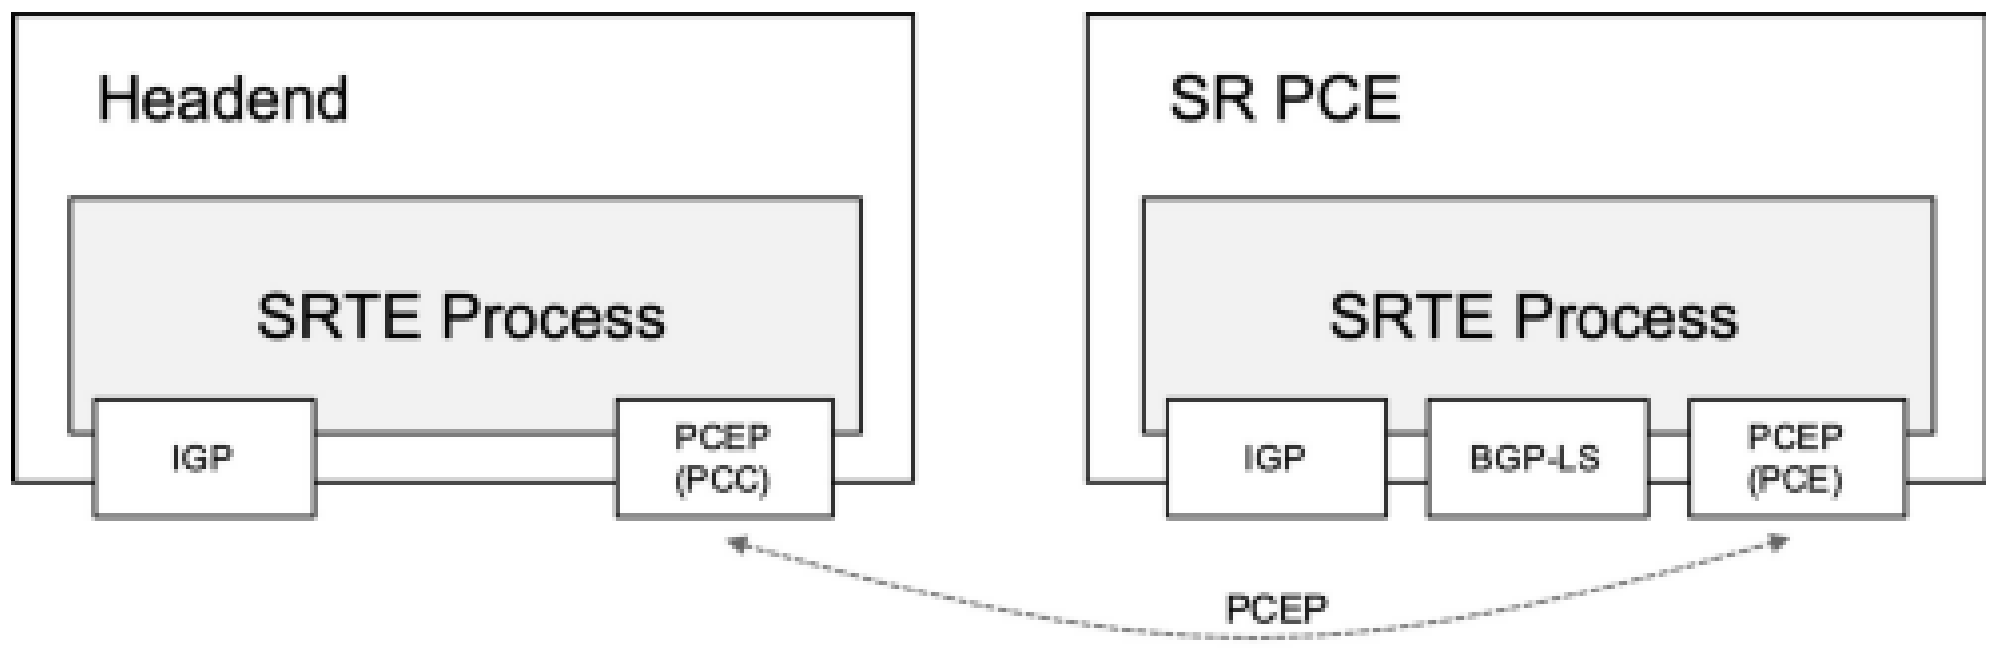
\includegraphics[width=\textwidth]{srte-headend-to-pce.png}
    \caption{SRTE Headend to PCE communication}
\end{figure}

\textbf{PCE -- Path Computation Element}

\vspace{5mm}
\noindent
A PCE provides a path computation service to other devices (PCCs) in the network, based on provided optimization objectives and constraints.
Path calculation can be initiated by the headend via stateless request/reply protocol exchange.
Once the ``delegation" bit is set by the headend, control of the path is then taken over by the PCE.

Path calculation can be initiated by the PCE or by an application via API.

PCE functionality can be enabled on any IOS XR device. However it is recommended to deploy separate nodes for PCE 
functionality to avoid the mixing of different functionality and enable better scalability.

Receives all topology information from different protocols 
(IS IS, OSPF, \href{https://www.noction.com/blog/bgp-ls-link-state}{BGP LS}) and combines them into the SR TE Database.

Link-delay metric is activated by default and available for policy computation.

\ttfamily distribute link-state \rmfamily command enables feeding SRTE DB by the routing protocol (OSPF and IS IS).

Redundancy/High Availability in PCE deployment is achieved with the following concepts:
\begin{itemize}
    \item Primary/Secondary PCE configuration: PCE configuration on any path calculation client is either designated as primary or secondary, enabling instant failover. 
    \item Topology learning: Using IGP / BGP information, all PCEs in the same network receive the same information about the topology present.
    \item SR Policy Reporting: When an SR Policy is instanciated, updated or deleted, the headend sends an \textbf{SR Policy State Report }to all its connected PCEs.
    \item Re-delegation behaviour: In case of failure of the primary PCE, all paths will be re-delegated to another PCE.   
    \item PCEP Keepalive/Dead Timer: PCEP Messages (keepalive or other) are sent at least every 30 seconds.
    \item Reachability of the PCE is tracked in every PCCs' forwarding table (no need to wait on any timers). 
    \item Inter-PCE State-Sync PCEP Session: An SR PCE can maintain PCEP sessions to other SR PCEs to indirectly distribute information in case some headend loses connection to one PCE. 
\end{itemize}

Split-brain situation when calculating disjoint-paths: path calculation can be impossible if one path is delegated to PCE1, and it
would have to be changed to calculate a disjoint path on PCE2. Creating a master/slave relationship between two PCEs solves this problem by only letting one 
of two PCEs calculate any disjoint path. 

\begin{figure}[]
    \centering
    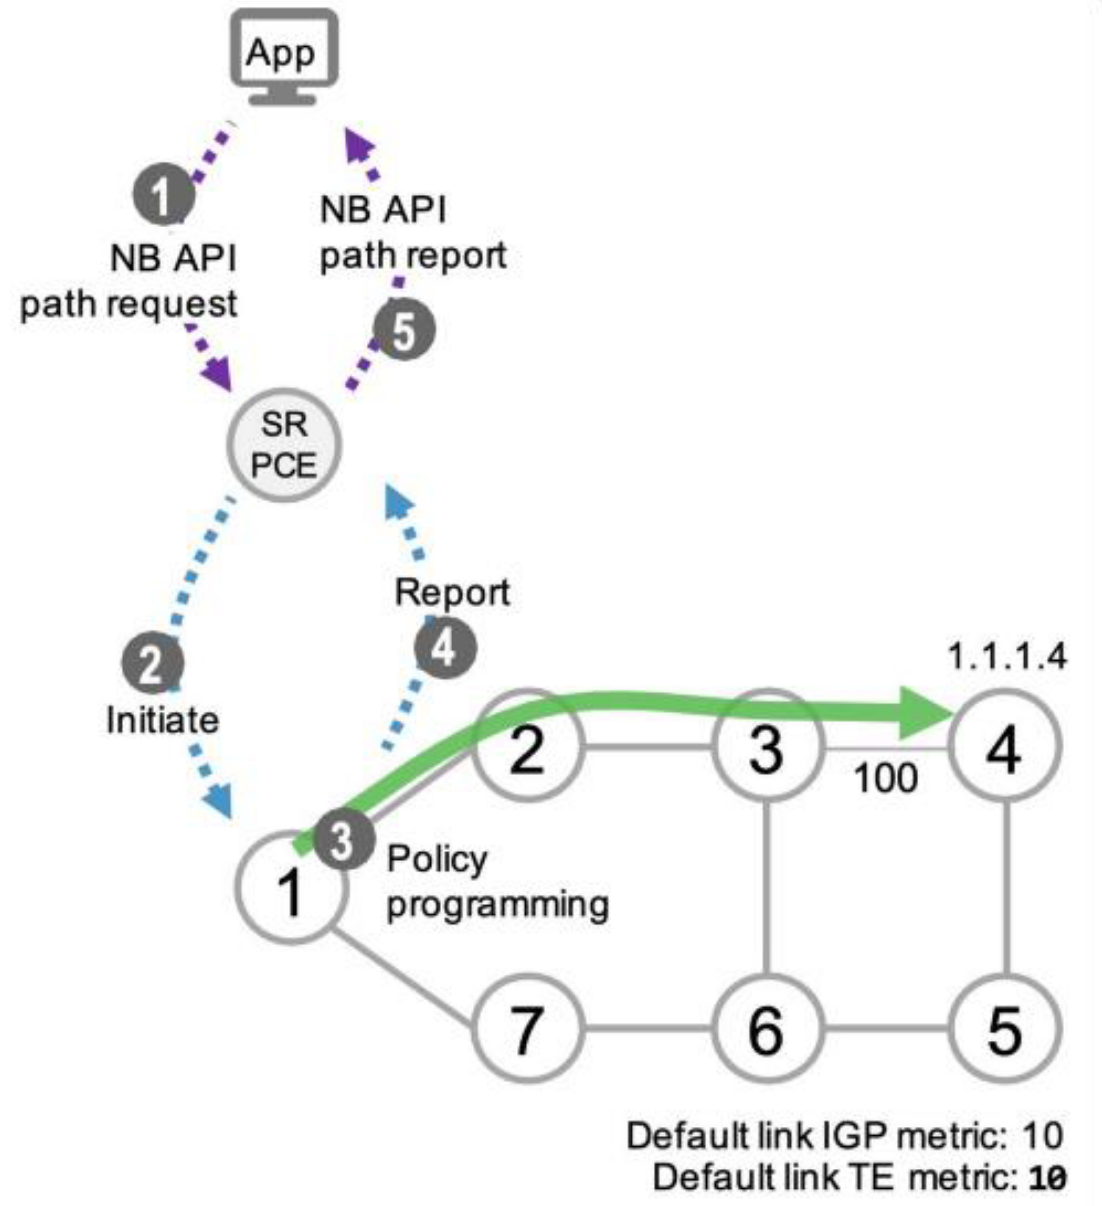
\includegraphics[width=8cm]{srte-arch.png}
    \caption{Basic SR TE Architecture}
\end{figure}

\textbf{Northbound Interface:} communicates with external applications, provides a structured endpoint 
to access and update topology and path information.

\textbf{Southbound Interface:} communicates with PCC devices, exchanging link state information and SR Paths. 

\subsection{LFA -- Loop Free Alternate}
\emph{``a directly connected neighbor that offers a repair path whose shortest path to the destination D does not traverse the protected component.''}

 
A suitable LFA does not always exist: it depends on the network topology, metrics and the component to be protected.

This is the reason LFA is usually topology dependent.

\begin{figure}
    \centering
    \includegraphics*[width=8cm]{srte-basic-lfa.png}
    \caption{LFA non-ideal repair path}
\end{figure}

\vspace{5mm} \noindent
The LFA basic Loop-free condition:
\emph{\[ ``Dist(N,D) < Dist(N,PLR) + Dist(PLR,D)" \]}
compares the length of the new path from the LFA (neighbor) to destination with the path from the LFA crossing the protected (failed) link.  

\vspace{5mm}
Point of Local Repair \textbf{(PLR)}: The Node that registered a link-down event and now has to adjust its path.

\textbf{N}: Node that is/has designated LFA path.

\subsubsection{TI-LFA: Topology Independent Loop-Free Alternate}

See also \href{https://www.segment-routing.net/tutorials/2016-09-27-topology-independent-lfa-ti-lfa/}{TI-LFA on segment-routing.net}

Offers node, link and Shared Risk Link Group SRLG protection with sub-50ms downtime. 100\% Coverage in any topology. Simple to operate and understand.
 Automatically computed by the IGP, no other protocol required.
 No state outside the protecting state at the PLR, local mechanism.
 Optimum: Backup path follows the post-convergence path. 
 Can be incrementally deployed
 Applies also to IP and LDP traffic (besides segment routing).

 
\vspace{5mm} \noindent
\textbf{Path Computation}: Calculate the shortest path with the outgoing link along the primary path pruned from the topology. 
Encode this path as a segment list to avoids microloops.

In a network with symmetric metrics, maximum two additional segments are required to form a valid repair path.

\begin{figure}[h]
    \centering
    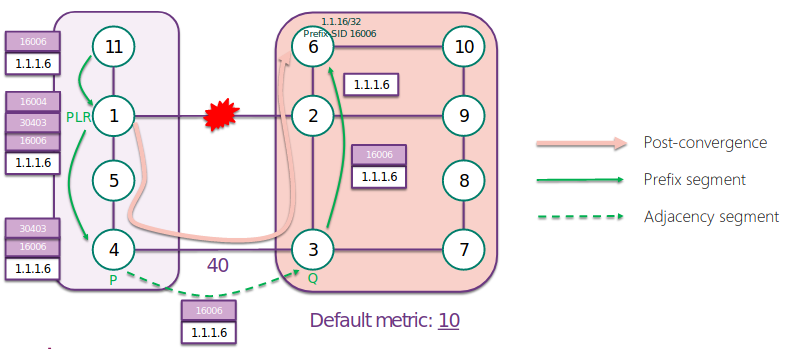
\includegraphics[width=\textwidth]{srte-tilfa.png}
    \caption{Repair Path using TI-LFA}
\end{figure}


\vspace{5mm} \noindent
Sample configuration for link protection:

\vspace{1mm} \noindent
\ttfamily
\noindent
router isis 1 \\
\hspace*{1em}address-family ipv4 unicast \\
\hspace*{2em}segment-routing mpls \\

\noindent
interface GigabitEthernet0/0/0/0 \\
\hspace*{1em}point-to-point \\
\hspace*{1em}address-family ipv4 unicast \\
\hspace*{2em}fast-reroute per-prefix \\
\hspace*{2em}fast-reroute per-prefix ti-lfa \\

\noindent
router ospf 1 \\
\hspace*{1em}segment-routing mpls \\
\hspace*{2em}fast-reroute per-prefix \\
\hspace*{2em}fast-reroute per-prefix ti-lfa enable  \\

\rmfamily